\chapter{M\'ODULOS, BLOQUES Y TEMAS}
\newpage
\section{Introducci\'on}
Se presenta una descripci\'on de las distintas extensiones que forman parte del \textit{i}CMS, de forma general las extensiones estan compuestas por m\'odulos, bloques y temas, veremos en detalle la estructura tanto a nivel de clases como a nivel de directorios. Al estar trabajando con un lenguaje de PostScripting como PHP, muchos de los archivos no aparecen en el modelo de clases, justamente por que no son clases como tal.

\section{Estructura de los m\'odulos}
Todos los m\'odulos siguen el patr\'on Modelo-Vista-Controlador, adem\'as maneja un archivo el cual se convierte en punto de entrada para el modulo, la finalidad de este archivo es para ejecutar el m\'etodo correcto del controlador dependiendo de la acci\'on requerida a trav\'es de los parametros del REQUEST.

\begin{figure}[h]
\centering
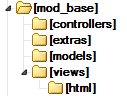
\includegraphics[scale=2, keepaspectratio=true]{imagenes/19_imagen.png}
\caption{Estructura de Directorios: M\'odulos. [Elaboraci\'on propia].}
\end{figure}

En el figura anterior el nombre del m\'odulo que utilizamos como ejemplo es ``base'', esta estructura de directorios es exactamente igual para todos los m\'odulos con la salvedad del nombre.\\
Dentro del directorio ``mod$\_$base'' tenemos una script php que sirve como punto de entrada al m\'odulo, adem\'as podemos ver que la unica finalidad de esta porci\'on de c\'odigo es recuperar una acci\'on y ejecutarla.\\

\begin{lstlisting}[label=jha_mod_base,caption=Punto de entrada al m\'odulo.]
<?php
...

$control = JhaRequest::getVar('controller', 'base');
require_once($GLOBALS['JHA_MODULE_PATH'].'controllers'.DS.$control.'.php' );

$classname = 'BaseController' . $control;
$controller = new $classname();

$controller->execute(JhaRequest::getVar('task'));
?>
\end{lstlisting}


Posteriormente tenemos al directorio ``extras'', el cual es utilizado generalmente para archivos auxiliares, tales como: Hojas de estilo y Javascript.

El directorio ``controllers'' se encarga de contener los controladores, por defecto siempre debe existir un archivo con el mismo nombre del m\'odulo, es decir un archivo llamado ``base.php''. Adem\'as los controladores siguen un patr\'on para definir el nombre de la clase, este patr\'on es: <<nombre$\_$modulo>>Controller<<nombre$\_$controlador>>, en el caso del controlador por defecto tenemos: ``BaseControllerBase'', si existiera un segundo controlador, por ejemplo ``block'' se tendr\'ia: ``BaseControllerBlock''.\\

El directorio ``models'' contiene todos los modelos, uno por cada controlador, la nomenclatura de sus nombres es muy similar a la de los controladores: <<nombre$\_$modulo>Model<nombre$\_$modelo>>, siendo <<nombre$\_$modelo>> exactamente el mismo que <<nombre$\_$controlador>>, entonces para el controlador ``base'' tenemos ``BaseModelBase'' y para ``block'' ``BaseModelBlock'' respectivamente.\\

El directorio ``views'' esta destinado a contener las vistas, igual que en el caso anterior una vista por cada controlador, le nomenclatura para los nombres es exactamente la misma que para los controladores y modelos, con la salvedad de que en vez de ``Controller'' y ``Model'' se utiliza ``View'', es decir: ``BaseViewBase'' y ``BaseViewBlock'' respectivamente.\\

Algo que es necesario mencionar es que una vista esta asociada a muchas plantillas (Plantilla no es lo mismo que Tema) para poder mostrar la informaci\'on bajo un formato determinado para cada caso, Paraesto utiliza el siguiente directorio.\\

El directorio ``html'' se encarga de contener las plantillas HTML, del cual se sirven las vistas para dar formato a la informaci\'on, estos archivos contienen en su mayoria (por no decir en su totalidad) contenido HTML con fragmentos de c\'odigo PHP unicamente.\\

\section{Estructura de los bloques}
Los bloques se registran en la base de datos, tienen en com\'un un campo llamado \textit{params} el cual sirve para establecer los parametros que definen como se debe mostrar\'a el contenido del bloque.\\
Por otro lado varios de los bloques, tienen un archivo denominado \textit{helper}, que se encarga de proveer funciones de acceso a datos y utilidades.\\
Todos los renderizadores de bloques llevan un archivo \textit{param.php}, el cual sirve para definir los parametros de cada bloque.\\

\section{Relaci\'on entre m\'odulos y bloques}
Los bloques y m\'odulos no guardan relaci\'on a nivel de c\'odigo, cada uno tiene una finalidad espec\'ifica.\\
Los m\'odulos procesan las interacciones del usuario con el sistema, es decir, que cada solicitud que el usuario hace al sistema es procesada a trav\'es de alg\'un m\'odulo. Como resultado de este procesamiento, se genera contenido HTML, el cual se ubica en una regi\'on particular de la plantilla a trav\'es de los renderizadores.\\
Los bloques por otro lado, solo se encargan de mostrar contenido, y lo hacen en regiones distintas a las del m\'odulo.

\section{M\'odulos}
A continuaci\'on vemos los distintos m\'odulos que forman parte de \textit{i}CMS.

\subsection{M\'odulo Base}
El m\'odulo base contiene funciones b\'asicas para el funcionamiento del CMS, tales como: la personalizaci\'on de la plantilla, agregado de nuevas plantillas, gestionado de bloques de contenido, configurado del CMS, entre otras.

\begin{figure}[h]
\centering
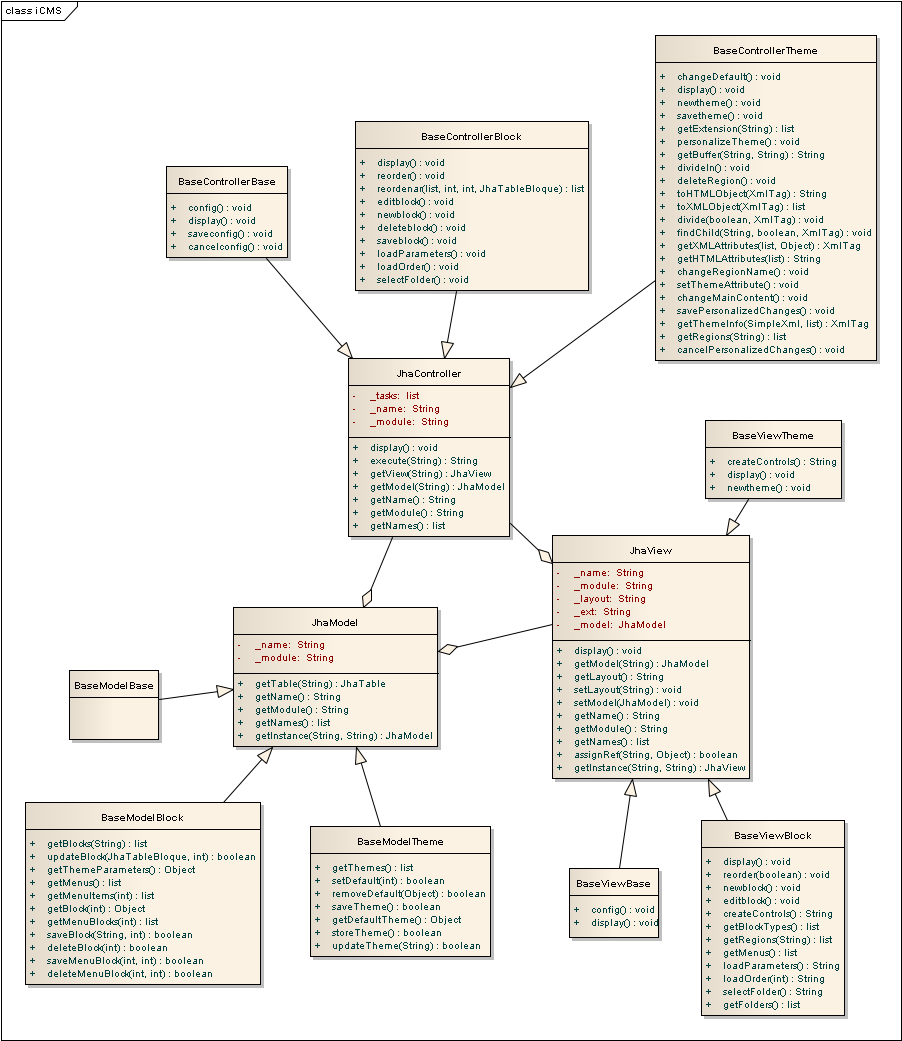
\includegraphics[scale=.35, keepaspectratio=true]{imagenes/13_imagen.png}
\caption{Modelo de clase: M\'odulo Base. [Elaboraci\'on propia].}
\end{figure}

\subsection{Configurado del CMS}
La configuraci\'on del CMS se hace a trav\'es del archivo \textit{JhaConfiguration}, gestiona los datos del servidor de base de datos as\'i como el prefijo de las tablas, tambi\'en se puede gestionar la vigencia de las noticias y tambi\'en los meta-datos para lo que se conoce como \textit{alta en buscadores}.

\subsection{Gesti\'on de plantillas}
La gesti\'on de plantillas comprende dos elementos importantes.\\
El primero de estos elementos, permite agregar nuevas plantillas e intercambiar la apariencia de la p\'agina a trav\'es de las plantillas.\\
Las plantillas que se suben al servidor deben tener una estructura concreta. Se deben tener m\'inimamente los siguientes archivos en un compreso ya sea tar.gz, tar.bz:
\begin{itemize}
\item index.php
\item info.xml
\item install.sql
\end{itemize}
\ldots\ Adicionalmente se pueden tener un directorio para im\'agenes y otro directorio para los css.\\
El segundo elemento permite personalizar la plantilla que se designa por defecto para mostrarse en el sitio. Para este efecto el m\'odulo provee mecanismos para ver las regiones definidas en la plantilla, asimismo tiene mecanismos para dividir las regiones ya sea en columnas o filas. Tambi\'en las regiones pueden moverse para reacomodar las regiones.\\
Este motor de gesti\'on de las plantillas provee una gama de opciones para que el usuario pueda personalizar a\'un m\'as su plantilla.

\subsection{Gesti\'on de bloques}
Los bloques son los contenidos secundarios, todos los bloques trabajan de forma muy similar, todas ellas tienen un renderizador espec\'ifico, en s\'intesis cada bloque tiene su propio renderizador.\\
A trav\'es de este gestor de bloques se definen elementos como la regi\'on donde se mostrar\'a el bloque, el orden entre bloques, y la relaci\'on entre los bloques y los men\'us, todo esto a nivel de administraci\'on avanzada del \textit{i}CMS, cuando hablamos de una administraci\'on est\'andar, hacemos referencia a los cambios que se pueden hacer directamente manipulando el contenido sobre la plantilla, o como decimos vulgarmente, ``En caliente''.

\subsection{M\'odulo Content}
El m\'odulo de contenido contiene funciones para el gestionamiento de las publicaciones del CMS, tales como: la gesti\'on de art\'iculos, gesti\'on de secciones y gesti\'on de noticias.

\begin{figure}[h]
\centering
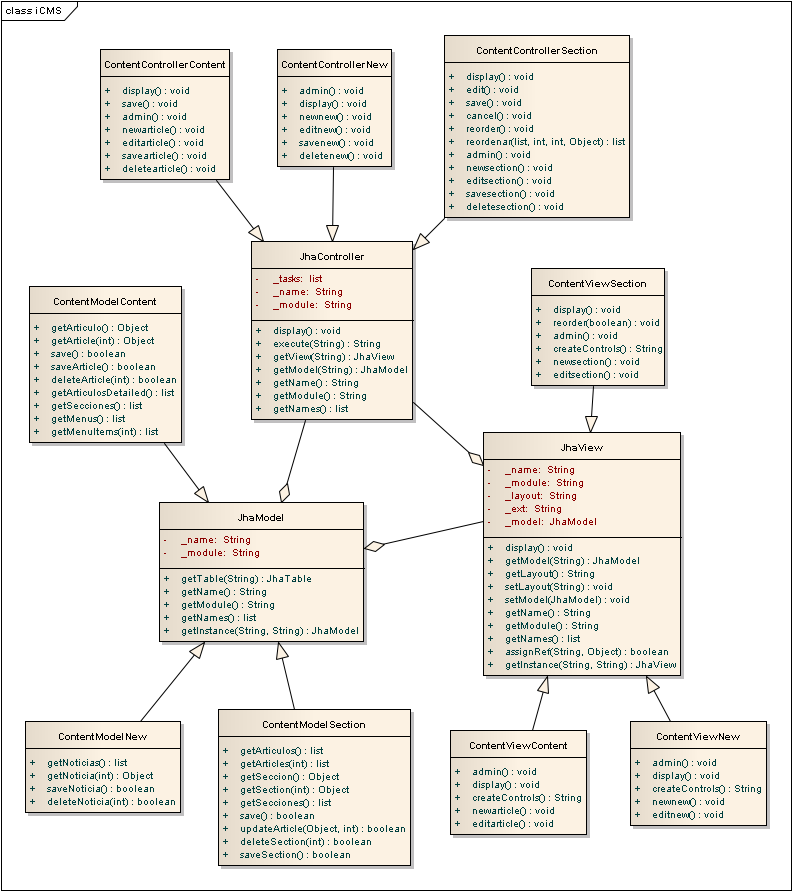
\includegraphics[scale=.4, keepaspectratio=true]{imagenes/14_imagen.png}
\caption{Modelo de clase: M\'odulo Content. [Elaboraci\'on propia].}
\end{figure}

\subsection{Gesti\'on de art\'iculos}
A trav\'es de este medio se pueden crear, editar, eliminar y listar los art\'iculos, los art\'iculos pertenecen a una secci\'on, adem\'as cada art\'iculo puede estar o no relacionado a un item de men\'u. Tambi\'en se cuenta con el editor WYSIWG para agregar el contenido de los art\'iculos.

\subsection{Gesti\'on de secciones}
Las secciones muestran un conjunto de art\'iculos al mismo tiempo, por el momento solo maneja una vista est\'andar de dos columnas, donde en la primera se muestra el art\'iculo mas reciente, y en la segunda se muestran los art\'iculos anteriores.\\
Las secciones al igual que los art\'iculos, tambi\'en estan relacionados a un enlace de men\'u.

\subsection{Gesti\'on de noticias}
Las noticias solo son p\'arrafos muy breves, avisos muy cortos que se sirven del bloque de noticias para mostrarse.\\
Al igual que la gesti\'on de secciones y art\'iculos se pueden crear, editar, listar y eliminar las noticias.

\newpage
\subsection{M\'odulo Men\'u}
El m\'odulo de men\'us contiene funciones para el gestionamiento de los men\'us del CMS.

\begin{figure}[h]
\centering
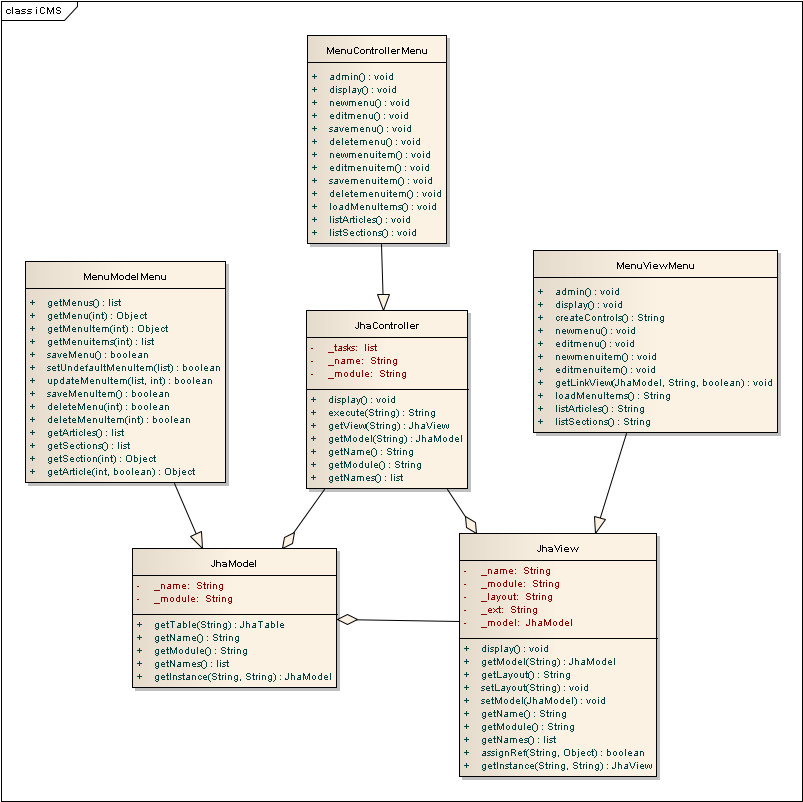
\includegraphics[scale=.4, keepaspectratio=true]{imagenes/15_imagen.png}
\caption{Modelo de clase: M\'odulo Men\'u. [Elaboraci\'on propia].}
\end{figure}

\subsection{Gesti\'on de men\'us}
La gesti\'on de men\'us contiene dos elementos: Los men\'us propiamente dichos y los \'items de men\'u.\\
Los men\'us solo agrupan un conjunto de \'items de men\'u.\\
Los \'items de men\'u contiene un enlace a art\'iculos, secciones o a p\'aginas externas al sitio, cada \'item de men\'u tiene un n\'umero de orden con respecto a los otros \'items del men\'u, tambi\'en pueden tener un \'icono asociado.

\subsection{M\'odulo User}
El m\'odulo de usuario contiene funciones para el gestionamiento de los usuarios del CMS.

\begin{figure}[h]
\centering
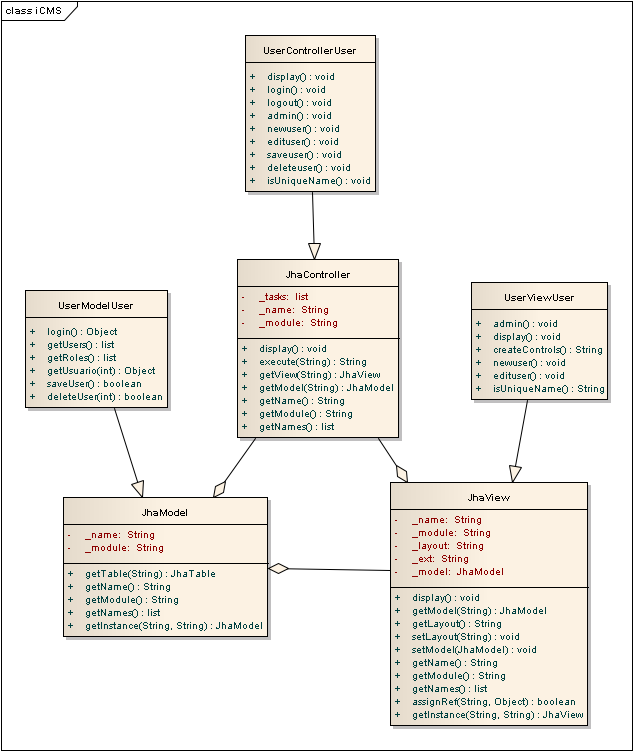
\includegraphics[scale=.4, keepaspectratio=true]{imagenes/16_imagen.png}
\caption{Modelo de clase: M\'odulo User. [Elaboraci\'on propia].}
\end{figure}

\subsection{Gesti\'on de usuarios}
A trav\'es de este gestor se pueden crear, modificar, eliminar y listar los usuarios registrados, los usuarios tienen roles definidos (Super Administrador, Editor) y el usuario visitante que no necesita registrarse. Dado que este CMS es un prototipo, no se contempla muchos de los datos de los usuarios.

\section{Bloques}
Como ya vimos en el cap\'itulo VI los bloques tienen renderizadores espec\'ificos, en este cap\'itulo veremos la especificaci\'on de cada uno de estos renderizadores de bloques.

\subsection{Bloque Banner}
Este renderizador sirve para mostrar banners de im\'agenes, estos banners dependiendo de los parametros del bloque pueden estar animados o no, los efectos son por defecto los que estan presentes en la librer\'ia \textit{effect} del \textit{framework jhaley} (sobreponer, entrar/salir vertical, entrar/salir horizontal).

\subsection{Bloque Breadcrumb}
El renderizador de la barra de navegaci\'on es bastante \'util, este renderizador crea los enlaces de la barra de navegaci\'on en funci\'on del men\'u, y va creaciendo con los enlaces de los art\'iculos.

\subsection{Bloque Custom}
Quiz\'as este renderizador sea el m\'as \'util, dado que la finalidad que tiene es de crear HTML personalizado. El HTML puede ser de cualquier tipo (im\'agenes, flash, etc.). Al momento de crear los bloques con este renderizador tambi\'en se crea el contenido HTML.

\subsection{Bloque Login}
Este renderizador tiene la finalidad de crear la ventana de acceso a las cuentas de usuario, el bloque de login trabaja en conjunto con el m\'odulo de usuario para validar los datos del usuario o tambi\'en para cerrar la sesi\'on del usuario

\subsection{Bloque Men\'u}
En cap\'itulos anteriores vimos el m\'odulo de men\'u, en el cual se gestiona los men\'us e \'items de men\'u, pues bien, este renderizador muestra los \'items de men\'u ordenados de acuerdo a un n\'umero de orden, cada bloque de men\'u puede acomodarse en men\'us verticales, horizontales, vertical en listas, tambi\'en es posible hacer visibles o no los iconos asociados a los \'items de men\'u.

\subsection{Bloque New}
Este renderizador trabaja en conjunto con el m\'odulo de contenido, concretamente con el gestor de noticias, este bloque solo se encarga de mostrar las noticias, las noticias pueden tener efectos animados dado que tambi\'en utilizan los efectos de la librer\'ia \textit{effect} del \textit{framework jhaley}.

\section{Temas}
En este cap\'itulo se tiene una descripci\'on de los temas que forman parte del CMS. Los temas o \textit{templates} son simplemente elementos que le dan al CMS la apariencia en funci\'on de los CSS e im\'agenes.\\
Por el momento se tiene dos temas creados especificamente para el CMS:

\begin{itemize}
\item \begin{description}
	\item[Tema Default] Este tema est\'a creado como apariencia por defecto del CMS
\end{description}
\item \begin{description}
	\item[Tema Enikma] Este tema es una alternativa de apariencia para el CMS.
\end{description}
\end{itemize}

\clearpage
